%\chapter{Введение в полулагранжевые методы для потоков геофизического масштаба} \label{chapt0}
\chapter{Введение} \label{chapt1}

Полулагранжевый метод является способом численного решения уравнений в частных производных, которые описывают процесс переноса. Данный метод учитывает лагранжевую природу процесса переноса, однако в тоже время, позволяет работать на фиксированной вычислительной сетке. Взяв за начало первые предложения в метеорологической литературе, которые фокусировались на переносе вихря в упрощенных моделях крупномасштабного потока, метод трансформировался в законченный метод дискретизации для полных уравнений атмосферных потоков. Полулагранжевый метод также связан (а, в некоторых случаях, полностью эквивалентен) с аналогичными методами, разработанными в других сферах моделирования, такими как, например, модифицированный метод характеристик, метод Эйлера-Лагранжа и характеристический метод Галеркина. 

Исчерпывающий обзор полулагранжевого метода в метеорологической литературе до 1990 года представлен в~\cite{A67}. Обзоры разработок, посвященных смежным методам в других областях моделирования, могут быть найдены, например, в~\cite{A15},~\cite{A43},~\cite{A56}.

Краткое описание данной вводной статьи представлено ниже. В разделе 2 представлена базовая концепция полулагранжевого метода, а также простейшие положения для линейного одномерного уравнения переноса. Кроме того, описаны разница и связь с сугубо лагранжевыми методами. В разделе 3, в ключе классического метео масштабного анализа, рассмотрена особая роль процесса переноса для крупномасштабного атмосферного потока. В разделе 4 кратко освещен процесс разработки полулагранжевых методов вкупе с некоторыми параллельными разработками в других научных сферах. В разделе 5 описаны некоторые из возможных способов реализации ключевых этапов в полулагранжевом методе. В разделе 6 представлены результаты простых численных тестов для одномерного и двумерного случая изолированного (passive) переноса с целью показать как метод может быть реализован на практике. Затем, результаты сравниваются с аналогичными эйлеровыми схемами. В разделе 7 обсуждается устойчивость и сходимость метода.

Первая версия данного обзора полулагранжевых методов была осуществлена, благодаря приглашению на семинар по прикладной математике на ETH Zurich, чтобы прочитать серию докладов по данной тематике в рамках программы ERCOFTAC в июле 2004. Я хотел бы поблагодарить профессоров Рольфа Джелтча (Rolf Jeltsch) и Уильяма Сойера (William Sawyer) за поддержку этого начинания и базовую концепцию данного обзора.

Мой первый персональный опыт работы с полулагранжевыми методами был получен в 1993 году в ходе моей работы над кандидатской диссертацией под руководством профессора Винчензо Касулли (Vincenzo Casulli, University of Trento, Italy). Я хотел бы поблагодарить его за мое посвящение как в данную восхитительную область, так и в мир практического численного моделирования. Всевозможные обсуждения с доктором Эндрю Станифортом (Andrew Staniforth, Met Office, UK) также были весьма важны в рамках углубления моего понимания обозначенных методов и проблем численного прогнозирования погоды в целом.

Мой опыт с полулагранжевыми методами также был углублен, благодаря обсуждениям и помощи моих многих друзей и коллег. Я хотел бы поблагодарить их всех за помощь и советы.

\newpage
%============================================================================================================================

\chapter{Полулагранжевый метод для линейного уравнения переноса} \label{chapt_2}
Для того, чтобы познакомиться с полулагранжевым методом в простом контексте, рассмотрим одномерное линейное уравнение переноса
%
\begin{equation}
\label{eq:equation2_1}
\frac{\partial c}{\partial t} + u\frac{\partial c}{\partial x} = 0
\end{equation}
%
с постоянным коэффициентом $u$ и с начальными данными $c_0(x), x\in{\mathbf{R}}$. Общеизвестно, что
%
\begin{equation}
\label{eq:equation2_2}
c(c,t)=c_0(x - ut)
\end{equation}
%
Теперь рассмотрим дискретизацию уравнения \eqref{eq:equation2_1} на равномерной одномерной сетке с шагом по пространству $\Delta x$ и временным шагом $\Delta t$. Обозначим узлы сетки как $i$, а дискретные временные уровни как $n$. Тогда пространственно-временные позиции на сетке могут быть обозначены $x_i=i\Delta{x}$, $t^n=n\Delta{t}$, а приближенные значения, вычисленные при помощи численного решения, как $c^n\approx c(x_i, t^n)$. Стандартные конечно-разностные методы основаны на аппроксимации дифференциальных операторов конечно-разностными приращениями. Рассмотрим некоторые типовые примеры. Одним из наиболее простых методов является противопотоковый метод, в котором для аппроксимации используются односторонние конечно-разностные приращения

%
\begin{equation}
\label{eq:equation2_3}
\frac{c_i^{n+1}-c_i^n}{\Delta t} + u\frac{c_i^n-c_{i-1}^{n}}{\Delta x} = 0
\end{equation}
%
Здесь предполагается, что $u\ge0$, а направление задано положительно (Here, it was assumed that u>=0 and the direction). Противопотоковый метод обладает первым порядком аппроксимации по времени и пространству. Информация о противопотоковых методах высокого порядка представлена, например, в~\cite{A12}. Метод с перешагиванием использует центральные конечные разности по времени и пространству
%
\begin{equation}
\label{eq:equation2_4}
\frac{c_i^{n+1}-c_i^{n-1}}{2\Delta t} + u\frac{c_{i+1}^n-c_{i-1}^{n}}{2\Delta x} = 0
\end{equation}
%
Итоговый метод имеет второй порядок аппроксимации по пространству и времени. Применение более точной аппроксимации пространственной производной может дать высокоточные схемы по пространству и времени. Например, взяв центральные разности по времени и аппроксимацию четвертого порядка производной по $x$ (например, см.~\cite{A14}), получим
%
\begin{equation}
\label{eq:equation2_5}
\frac{c_i^{n+1}-c_i^{n-1}}{2\Delta t} + u\Big[\frac{4}{3}\frac{c_{i+1}^n-c_{i-1}^n}{2\Delta x}-\frac{1}{3}\frac{c_{i+2}^n-c_{i-2}^n}{4\Delta x}\Big] = 0.
\end{equation}
%
Упомянутые методы являются трехшаговыми по времени, потому требуют использования особой аппроксимации для вычисления первого шага по времени. Примером двухшагового по времени метода, который имеет второй порядок аппроксимации, является метод Лакса"--~Вендроффа
%
\begin{equation}
\label{eq:equation2_6}
\frac{c_i^{n+1}-c_i^n}{\Delta t} + u\frac{c_i^n-c_{i-1}^n}{2\Delta x} - \frac{u^2\Delta t}{2}\frac{c_{i+1}^n-2c_i^n+c_{i-1}^n}{\Delta x^2} = 0,
\end{equation}
%
который может быть  интерпретирован как устойчивая версия (неустойчивой) схемы
%
\begin{equation}
\label{eq:equation2_7}
\frac{c_i^{n+1}-c_i^n}{\Delta t} + u\frac{c_{i+1}^n-c_{i-1}^n}{2\Delta x} = 0,
\end{equation}
%
полученной добавлением численной диссипации в особом виде (например, см.~\cite{A56}). Общеизвестно, что устойчивость этих методов зависит в основном от параметра $C=u\Delta t/\Delta x$, также известного как число Куранта. Основное условие для устойчивости это, фактически, $\left|C\right|\le1$, которое также известно как условие Куранта"--~Фридрихса"--~Леви (КФЛ) (см.~\cite{A10}).

Лагранжевые и полулагранжевые методы, в свою очередь, используют характерную особенность уравнения переноса, а именно представление точного решения через начальные данные. В частности, рассмотрев без потери общности случай $u\ge0$, можно обнаружить, что имеют место два следующих уравнения
%
\begin{equation}
\label{eq:equation2_8}
\begin{split}
c (x_i, t^n) & = c_0(x_i - un\Delta t) {} \\
		     & {} = c_0(x_i + u\Delta t - u(n+1)\Delta t) = c(x_i + u\Delta t, t^{n+1})
\end{split}
\end{equation}
%
%
\begin{equation}
\label{eq:equation2_9}
\begin{split}
c (x_i, t^{n+1}) & = c_0(x_i - u(n+1)\Delta t) {} \\
& {} = c_0(x_i - u\Delta t - un\Delta t) = c(x_i - u\Delta t, t^{n})
\end{split}
\end{equation}
%
Уравнение \eqref{eq:equation2_9} является основой для чистых лагранжевых методов. Особая природа точного решения уравнения \eqref{eq:equation2_1} позволяет использовать информацию о решении в точке сетки в момент времени $n$, чтобы вывести значение решения в момент времени $n+1$ в точках сетки, которые \textit{переместились с потоком}. В результате того, что сетку необходимо менять на каждом временном шаге, практическое приложение лагранжевых методов неэффективно и данные методы никогда не становились действующими (operational) инструментами в прогнозе погоды или крупномасштабных атмосферных симуляциях.

Уравнение \eqref{eq:equation2_10} обеспечивает основу для полулагранжевого метода. Вновь используется особая природа точного решения \eqref{eq:equation2_1}, чтобы выразить значение решения в узлах сетки на временном шаге $n+1$ через значения решения на временном шаге $n$ в тех узлах сетки, которые \textit{будут перенесены потоком} на вычислительную сетку за один временной шаг.
Тот факт, что сетка не изменяется во времени, имеет практическое преимущество, которое является одной из фундаментальных причин для гораздо более широкого использования полулагранжевых методов, нежели чисто лагранжевых. Дискретное определение полулагранжевого метода может быть получено из уравнения \eqref{eq:equation2_10} (\textbf{ТУТ ЯВНАЯ ОШИБКА, видимо имеется ввиду некоторое уравнение представленное выше}) как
%
\begin{equation}
\label{eq:equation2_10}
c_i^{n+1} = c_{i-u\frac{\Delta t}{\Delta x}}^{n} = c_{i-k-\alpha}^n \quad u\frac{\Delta t}{\Delta x} = k + \alpha \quad k = \Big[u\frac{\Delta t}{\Delta x}\Big].
\end{equation}
%

$k$ and $\alpha$ часто называют целым и дробным числами Куранта, соответственно. Выражение $c_{i-k-\alpha}^n$ может быть интерпретировано как значение, полученное из приближенных значений $c^n$ в точке $i\Delta x - u\Delta t$ с использованием некоторой интерполяционной процедуры. Применив линейную интерполяцию, можно сразу получить два интересных факта
%
\begin{equation}
\label{eq:equation2_11}
c_i^{n+1} = \alpha c_{i-k-1}^{n} + (1-\alpha)c_{i-k}^n.
\end{equation}
%
Во первых, если $C = u\Delta t/\Delta x < 1$, тогда имеем в \eqref{eq:equation2_11} $k=0$, $C=\alpha$ и  легко увидеть, что итоговый метод идентичен противопотоковому методу \eqref{eq:equation2_3}. Более того, ясно, что \eqref{eq:equation2_11} выполняется для любого значения числа Куранта и что, поскольку значения решения на новом временном слое $n+1$ получены с использованием линейной интерполяции значений на временном слое $n$ с неотрицательными коэффициентами, выполняется дискретный принцип максимума, т. е.
%
\begin{equation}
\label{eq:equation2_12}
\min_i c_i^0 \le \min_i c_i^n \le \max_i c_i^n \le \max_i c_i^0
\end{equation}
%
для любого $n$. Это также подразумевает устойчивость в максимум-норме для произвольного числа Куранта. Таким образом, по крайней мере в простом случае, полулагранжевый метод, очевидно, имеет большое преимущество над рассмотренными ранее эйлеровыми методами, поскольку отсутствует условие устойчивости, ограничивающее выбор временного шага.

Полулагранжевый метод может быть легко обобщен на многомерный случай. Рассмотрим поле постоянных скоростей $\mathbf{u}\in\mathbf{R}^d$ и начальное условие $c_0(x), x\in\mathbf{R}^d$. Тогда многомерное линейное уравнение адвекции имеет вид
%
\begin{equation}
\label{eq:equation2_13}
\frac{\partial{c}}{\partial{t}} + \mathbf{u} \cdot \nabla c = 0.
\end{equation}
%
Как и в одномерном случае, аналитическое решение представимо в виде
%
\begin{equation}
\label{eq:equation2_14}
c(\mathbf{x}, t) = c_0(\mathbf{x} - \mathbf{u}t),
\end{equation}
%
и полулагранжевый метод может быть выведен как и в одномерном случае, лишь заменив одномерную интерполяцию на многомерную.
	
В более общем случае, когда поле скоростей $\mathbf{u} (\mathbf{x},t)\in\mathbf{R}^d$ зависит от пространства и времени, имеем
%
\begin{equation}
\label{eq:equation2_15}
\frac{dc}{dt}=\frac{\partial{c}}{\partial{t}} + \mathbf{u}(\mathbf{x}, t) \cdot \nabla c = 0.
\end{equation}
%
Здесь была введена обычная запись $dc/dt$ для обозначения лагранжевой производной. Полагая, для поля скоростей верны некоторые предположения о непрерывности (оно должно быть непрерывным по Липшицу, например, см.~\cite{A56}), можно доказать, что существует функция линий тока или характеристическая функция. Они определены как решения $\mathbf{X}(t;s, \mathbf{x})$ обыкновенных дифференциальных уравнений
%
\begin{equation}
\label{eq:equation2_16}
\frac{d}{dt}\mathbf{X}(t;s,\mathbf{x})=\mathbf{u}(\mathbf{X}(t; s, \mathbf{x}), t)
\end{equation}
%
с начальным условием в момент времени $s$, заданным как $\mathbf{X}(t;s,\mathbf{x})=\mathbf{x}$. Для гладких начальных данных по цепному правилу доказуемо, что
%
\begin{equation}
\label{eq:equation2_17}
c(\mathbf{x}, t) = c_0(\mathbf{X}(0;t,\mathbf{x})).
\end{equation}
%
Это показывает, что доказательство, аналогичное упомянутому, справедливо для численного метода основанного на полулагранжевом подходе, однако при условии, что получено численное решение уравнения \eqref{eq:equation2_16}. Таким образом, подводя итог, можно сказать, что, используя формулу \eqref{eq:equation2_17}, полулагранжевые методы сводят аппроксимацию уравнения переноса \eqref{eq:equation2_15} к следующим ключевым шагам:
\begin{itemize}
	\item на заданном слое по времени $n$, для каждой точки сетки $x$ вычислить приближенное решение \eqref{eq:equation2_16} для определения оценки $\mathbf{X}^*(t^n;t^{n+1}, \mathbf{x})$
	\item вычислить аппроксимацию уравнения \eqref{eq:equation2_17} путем интерполяции значений в узлах сетки на временном слое $n$ в точках $\mathbf{X}^*(t^n;t^{n+1}, \mathbf{x})$.
\end{itemize}
Это подразумевает что решение ДУЧП \eqref{eq:equation2_15} сведено к решению большого набора взаимно независимых ОДУ и многомерной интерполяции. Для каждого из этих шагов доступен ряд классических и хорошо изученных методов.
\newpage
\chapter{Роль адвекции в потоках геофизических масштабов} \label{chapt_3}
Уравнения Эйлера во вращающейся системе координат могут быть записаны как
%
\begin{align}
\label{eq:equation3_1}
\frac{d\rho}{dt}&=-\rho\nabla\cdot\mathbf{u}\\
\label{eq:equation3_2}
\frac{d\mathbf{u}}{dt}&=-\frac{1}{\rho}\nabla p - 2 \mathbf{\Omega} \times \mathbf{u} - \nabla \Phi\\
\label{eq:equation3_3}
c_v\frac{dT}{dt}&=-p\nabla\cdot\mathbf{u}.
\end{align}
%
Для крупномасштабного атмосферного движения, горизонтальный пространственный масштаб $L=\mathcal{O}(10^7)m$ намного больше, чем вертикальный масштаб $D=\mathcal{O}(10^4)m$. Вследствие этого гидростатическое допущение является хорошей аппроксимацией (см. например,~\cite{A24},~\cite{A49} касательно полного вывода масштабного анализа). Более того, многие ключевые динамические особенности решения полной системы учитываются упрощенными моделями, которые могут быть получены при использовании баротропического допущения $p=p(\rho)$ и при  рассмотрении вертикального среднего уравнений в отношении однородного слоя жидкости переменной глубины. Данное допущение снова основано на том факте, что $L >> D$ и это приводит нас к двумерной модели, также известной как "уравнения мелкой воды"
%
\begin{equation}
\label{eq:equation3_4}
\frac{dh}{dt}=-h\nabla \cdot \mathbf{v}
\end{equation}
%
%
\begin{equation}
\label{eq:equation3_5}
\frac{d\mathbf{v}}{dt}=-g\nabla h - f\mathbf{k}\times \mathbf{v}.
\end{equation}
%
где $f=2\Omega\sin\theta$, $\theta$ это широта, а орографический профиль взят за константу. Если взять ротор уравнения количества движения и скомбинировать результат с уравнением неразрывности, то получим так называемое уравнение потенциальной завихренности
%
\begin{equation}
\label{eq:equation3_6}
\frac{d}{dt}\Big(\frac{\zeta + f}{h}\Big) = 0.
\end{equation}
%
Общепризнанно, что уравнение \eqref{eq:equation3_6} является решением большинства крупномасштабных волн (волны Россби) которые представляют собой огромные метеорологические системы. Дальнейшее упрощение может даже привести к квазигеострофической модели, в которой разновидность уравнения \eqref{eq:equation3_6} является, по сути, прогнозирующим уравнением, а все остальные эволюционные уравнения заменены на приближенные балансовые соотношения. Начиная с основополагающей работы~\cite{A8}, ранние модели численного предсказания погоды (см., например,~\cite{A24},~\cite{A73}) использовали данную упрощенную систему по ряду причин вычислительного характера. Точное решение уравнения \eqref{eq:equation3_6} (или решение эквивалентных формулировок вихревой адвекции) суть одна из неотъемлемых особенностей для моделей, предназначенных для симуляции крупномасштабных атмосферных потоков. Именно в данном контексте, был впервые разработан полулагранжевый подход и, спустя годы, стал распространённым методом численного моделирования.

Необходимо отметить, что, несмотря на концептуальные причины, существовало большое количество практических стимулов к успешному применению полулагранжевых методов в метеорологии. На стандартных декартовых сетках при использовании сферических координат, сближение меридианов на полюсах приводило к очень большим числам Куранта, даже при достаточно разреженной (в остальной области) вычислительной сетке. Данная особенность, известная также как "полюсная проблема", приводит к необходимости специально обрабатывать полюсные "шапочки" (pole caps) во многих глобальных моделях. Полулагранжевые методы, будучи безусловно устойчивыми, не представляют никаких особенных проблем в этом отношении. Однако, указанные методы по-прежнему требуют подходящего подхода к координатной сингулярности при расчете траекторий и при к интерполяции в ячейках, близких к полюсам.
\chapter{Историческое развитие полулагранжевых методов} \label{chapt_4}
Первой статьей, посвященной методам для уравнения переноса и методам, которые применяют подход распространения вдоль характеристик, является хорошо известная работа Куранта, Айзексона и Риз~\cite{A11} по численному решению гиперболических систем, а в метеорологической литературе, статья о методике графического интегрирования Р. Фьортофта~\cite{A20}. Более детальный анализ был проведен Виин"=Нильсеном в~\cite{A73}. В этой статье, снова внимание было уделено баротропическому вихревому уравнению, которое представляло собой единственную модель с помощью которой в то время мог быть получен практически значимый численный прогноз. Затем этот метод был применен в~\cite{A48}, а затем переформулирован в тот вид, который весьма похож на тот, что применяется сегодня. Первое применение к простейшей модели уравнения переноса было представлено в~\cite{A28}, а первое подтверждение того, что большие шаги по времени могут быть использованы в методе без появления численной неустойчивости решения, было найдено Дж. Сойером в~\cite{A63}. Дальнейшая разработка метода характеристик проводилась в~\cite{A1}, в тоже время, дальнейший анализ и тесты в метеорологической литературе проводились в~\cite{A30},~\cite{A12}. Как отмечалось ранее, одна из особенностей, которая на сегодняшний день наиболее тесно ассоциируется с полулагранжевыми методами, а именно свойство сохранять устойчивость при любом числе Куранта, в то время не являлась столь очевидной. (см., например,~\cite{A30},~\cite{A53}).

В ранних восьмидесятых, разнообразные публикации упрочнили роль полулагранжевых методов (а также методов, основанных на характеристиках) в разных подходах к моделированию. В области конечных элементов, огромное влияние оказали статьи Пирону~\cite{A50} и Дугласа~\cite{A27}. В области конечно-объемных подходов, Д. Моретти в~\cite{A41} была предложена разновидность метода характеристик. Также К. В. Мортоном в~\cite{A42},~\cite{A45} была введена концепция характеристических методов Галеркина. В контексте метеорологии, ключевыми являются работы~\cite{A59},~\cite{A60} A. Роберта, в которых был пересмотрен численный метод Сойера и затем объединен с техникой полу"=неявной дискретизации, таким образом демонстрируя полный потенциал полулагранжевых методов с точки зрения использования гораздо более больших шагов по времени. Лежащая в основе полулагранжевого подхода безусловная сходимость для линейной и квадратичной интерполяции на декартовых сетках была доказана Дж. Р. Бейтсом и А. Макдональдом в~\cite{A3}. Анализ устойчивости кубической сплайн интерполяции на декартовых сетках из~\cite{A53} был расширен А. Станифортом и К. Темпертоном в~\cite{A52} на случай для чисел Куранта больше единицы. Двухшаговые схемы были предложены А. Макдональдом и Дж. Р. Бейтсом в~\cite{A38}, а также А. Станифортом и К. Темпертоном в~\cite{A70}. Связка полулагранжевых методов с методами спектрального анализа для простейших уравнений движения была впервые предложена Г. Ритчи в~\cite{A57},~\cite{A58}. Общая устойчивость и анализ сходимости для случая адвекции с переменными коэффициентами была представлена в~\cite{A16} в контексте конечно-элементной формулировки.

В 2000 году ситуация такова, что ряд оперативных центров используют полулагранжевые модели для своих дневных прогнозов. Среди этих моделей можно выделить, например, IFS (Integrated Forecast System) в ECMWF (European Centre for Medium-Range Weather Forecasts)~\cite{A71}, GEM (Global Environmental Multiscale Model) модель в RPN Canada (The Recherche en Prévision Numérique)~\cite{A9} и Universal Model в Met Office~\cite{A72}.
\chapter{Практика полулагранжевых методов} \label{chapt_5}
Как было показано в разделе 2, полулагранжевые методы сводят аппроксимацию уравнения \eqref{eq:equation2_15} к следующим двум ключевым этапам:
\begin{itemize}
	\item на заданном слое по времени $n$, для каждой точки сетки $x$ вычислить приближенное решение \eqref{eq:equation2_16} для определения оценки $\mathbf{X}^*(t^n;t^{n+1}, \mathbf{x})$
	\item вычислить аппроксимацию уравнения \eqref{eq:equation2_17} путем интерполяции значений в узлах сетки на временном слое $n$ в точках $\mathbf{X}^*(t^n;t^{n+1}, \mathbf{x})$.
\end{itemize}
Ниже обсудим как получить решение на каждом этих этапов и достичь, при этом, великолепной точности и эффективности в итоговом численном методе.
\section*{Подходы к аппроксимации траекторий} \label{sect5_1}
Аппроксимацией уравнения
%
\begin{equation}
\label{eq:equation5_1}
\frac{d}{dt}\mathbf{X}(t;t^{n+1},x) = \mathbf{u}\Big(\mathbf{X}(t;t^{n+1}, x),t\Big)
\end{equation}
%
с начальными данными $\mathbf{X}(t;t^{n+1},\mathbf{x})=\mathbf{x}$ на слое $t^{n+1}$ по существу является решатель, который дает приближенные обратные лагранжевые траектории, опущенные из точек сетки. Важно заметить, что решение \eqref{eq:equation5_1} требует, вообще говоря, чтобы поле скоростей было известно в точках, которые не принадлежат пространственно-временной сетке. Применительно к реальным моделям, это означает, что необходима некоторая интерполяция (а касательно зависимости по времени --- экстраполяция). Традиционно, используются три основных стратегии для аппроксимации траекторий частиц:
\begin{itemize}
	\item подход с итерацией по неподвижной точке (fixed point operational approach)
	\item метод расщепления с явными решателями ОДУ (substepping with explicit ODE solvers)
	\item разложение в ряд Тейлора с параметрическим представлением для траектории (Taylor expansion of the parametric representation for the trajectory)
\end{itemize}
Итерация по неподвижной точке в наиболее общеизвестной виде была представлена в~\cite{A59}, хотя итерационный метод также использовался в~\cite{A36}. Это наиболее широко признанный (можно сказать, почти единственно признанный) метод в моделировании атмосферы. Определяя перемещение $\mathbf{a}=\mathbf{x} - \mathbf{X}(t^n;t^{n+1}, \mathbf{x})$ как искомую неизвестную величину, метод Роберта состоит в формулировании уравнения перемещения
%
\begin{equation}
\label{eq:equation5_2}
	\mathbf{a}=\Delta t \mathbf{u}(\mathbf{x} - \mathbf{a}, t^*),
\end{equation}
%
где $t^*$ это время на которое поле скоростей было остановлено, чтобы вычислить траекторию. В зависимости от значения $t^*$, достигается более или менее точная дискретизация по времени, см., например, обсуждение в []. Например, для того, чтобы получить второй порядок точности дискретизации по времени, в случае двухшаговой схемы, следует выбрать $t^*=t^{n+\frac{1}{2}}$, что приводит к необходимости временной экстраполяции в случае, когда поля скоростей известны только до времени $t^n$ включительно. Преимущество итерационного подхода заключается в том, что он безусловно устойчив, а также в том, что может быть доказана итерационная сходимость при относительно не жестких условиях для атмосферных потоков, см., например,~\cite{A52},~\cite{A65}.

С другой стороны, методы траекторий более популярны в конечно-элементном моделировании, а также в моделировании прибрежных зон (см., например,~\cite{A50},~\cite{A7},~\cite{A56},~\cite{A16},~\cite{A40}). Тем не менее, использование данных методов в приложении к атмосферным моделям также описано в литературе, см., например,~\cite{A6},~\cite{A22}. Чтобы гарантировать тот факт, что приближенные траектории не пересекают друг друга, всякий раз, когда число Куранта больше единицы, для их аппроксимации, как правило, используют более мелкие шаги по времени.

В качестве альтернативного подхода, в~\cite{A39} был предложен метод разложения в ряд Тейлора для декартовых сеток, который был затем расширен на сетки с треугольными конечными элементами. Данный метод основывается на разложении $\mathbf{X}(t^n,t^{n+1},\mathbf{x})$ в ряд Тейлора по времени и последующей аппроксимации полученных производных. Преимущество данного метода над озвученными выше заключается в том, что он не требует интерполяций или экстраполяций. С другой стороны, аппроксимированная производная по времени требует дополнительной памяти, а взятие производной от аппроксимации суть полностью эвристический процесс и, в общем случае, не корректен для определенных потоков.

Другим возможным подходом, который был предложен Р. Д. Персером и Л. М. Лесли в~\cite{A55}, является использование опережающих траекторий.
\section*{Методы интерполяции} \label{sect5_2}
Другим ключевым ингредиентом при реализации полулагранжевого метода является процедура интерполяции, используемая на каждом временном шаге для восстановления значений решения в исходной точке линии тока. Принимая во внимание контекст в котором разрабатывались полулагранжевые методы, достаточно легко объясняется большое количество работ по оценке свойств интерполяционных алгоритмов для декартовых сеток. Как будет показано в разделе 6, линейная интерполяция продуцирует весьма диффузивные решения. 
% In the case of one dimensional flow with Courant numbers smaller than one, it is easy to see that in fact the upwind method is recovered. 
% Не совсем понятное предложение. Здесь наверняка подразумевается, что линейная интерполяция дает первый порядок аппроксимации, но не уверен.
Легко увидеть, что в случае одномерного потока с числами Куранта меньшими единицы, данная интерполяция дает фактически результаты метода набегающего потока. Квадратичная интерполяция использована в~\cite{A3}. Кубическая  интерполяция Лагранжа использовалась в~\cite{A63}. В~\cite{A53} впервые применена кубическая сплайновая интерполяция. Кубическая интерполяция Лагранжа также использована в фундаментальных работах Роберта~\cite{A59},~\cite{A60} и проанализирована в~\cite{A52}. Данный метод интерполяции наиболее широко используется в атмосферных прикладных задачах. Как было показано Маккалпином в~\cite{A37}, в общем случае возможно получить различные свойства в зависимости от того факта, полиномы какого порядка (четного или нечетного) использовались для интерполяции. Также, Р. Д. Персером в~\cite{A54} был предложен так называемый каскадный метод интерполяции. Улучшенная версия каскадного метод интерполяции представлена в~\cite{A46}.

На неструктурированных сетках, типичных для конечно-элементных моделей, в основном используется конечно-элементные интерполяторы. Однако, в~\cite{A61},~\cite{A62},~\cite{A4} было доложено об успешных попытках в достижении высокой точности при помощи кригинга, а также интерполяторов на основе радиальных базисных функций.
%Kriging is a group of geostatistical techniques to interpolate the value of a random field (e.g., the elevation, z, of the landscape as a function of the geographic location) at an unobserved location from observations of its value at nearby locations


Общеизвестно, что принцип максимума, обсуждавшийся в разделе 2 для случая линейной интерполяции, не может быть доказан для случая интерполяторов высокого порядка. Данная ситуация аналогична тем, которые имеют место быть для многих других численных схем решения уравнения переноса, см., например,~\cite{A32},~\cite{A56}. Данный аспект рассматривается в~\cite{A74}, где сравниваются различные методы монотонной интерполяции (основанные на эрмитовой интерполяции). Основные рекомендации по преодолению внутренней нехватки монотонности всех интерполяций высокого порядка и монотонизации полулагранжевого метода вместе с доказательством монотонности полученной схемы приведены в~\cite{A5}. Данный подход также широко применяется в реальных задачах операционных центров.
% имеются ввиду центры погоды.
Для всех экспериментов, осуществленных в разделе 6, рассматриваются гладкие решения (для которых минимизированы выбросы и вбросы (overshoots, overshoots)) без использования процедур монотонизации.
\chapter{Численные эксперименты: одно- и двумерный пассивный перенос} \label{chapt_6}
В данной главе будут представлены результаты некоторых численных экспериментов с целью дать представление о том, как работает полулагранжевый метод и как может быть получена разная точность путем варьирования алгоритмов интерполяции и аппроксимации траекторий. В контексте некоторого базового сравнения двух подходов также будут представлены результаты аналогичных тестов при использовании эйлеровых схем. Хотелось бы обратить внимание на то, что хорошие результаты вычислений для модельных тестовых случаев является необходимым, но не достаточным условием для общей применимости численного метода. Более того, неудовлетворительные результаты не отменяют применимости в особых случаях, отличных от рассматриваемого, и не всегда представляется возможным дать общее заключение, исходя из рассмотренных частных случаев. Наконец, что не менее важно, оценка эффективности конкретного метода, согласно нашему представлению, может быть осуществлена только очень приблизительно, поскольку итоговое время счета сильно зависит от многих условий, которые имеют мало общего с самим численным методом (например, стиль кодирования и архитектура процессора). Хотя эти соображения продиктованы лишь здравым смыслом, их свойственно игнорировать, когда различные философии моделирования сравниваются между собой в упрощенном контексте.
\section*{Одномерная адвекция} \label{sect6_1}
Были проведены одномерные эксперименты на интервале $[0, 2]$ для уравнения \eqref{eq:equation2_1}, в качестве начальных данных выбрана финитная колоколообразная функция $\mathcal{C}^1$ с максимальным значением равным 10. Скорость адвекции $u=1/2$, а шаг по пространству был $\Delta x=1/100$. Для первых экспериментов, шаг по времени $\Delta t = 0.05$, таким образом число Куранта было зафиксировано как $C=2.5$. Тест проводился до времени $T=2$. Полученные результаты для полулагранжевого метода, использующие линейную, квадратичную и кубическую интерполяцию показаны на графиках \ref{img:6_1}, \ref{img:6_2}, \ref{img:6_3}, соответственно (черные линии использованы для начальных данных, серые линии показывают конечное время). Следует отметить, что в данном тесте использовалось точное значение исходной точки траектории, поскольку все основные схемы интегрирования дали бы точное решение в простейшем случае постоянной скорости в пространстве и времени.
%
\begin{figure}[ht] 
	\centering
	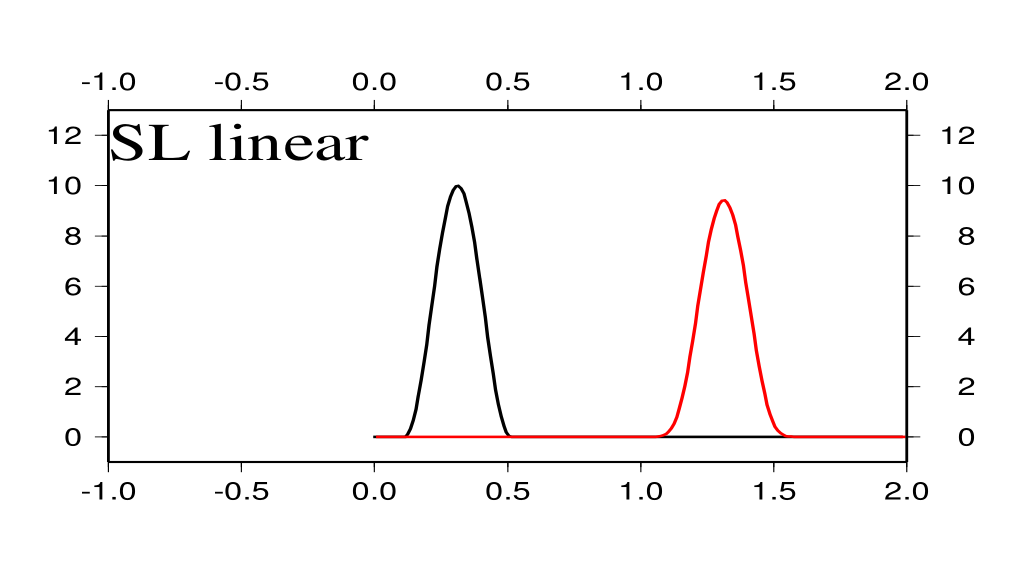
\includegraphics[width=0.8\textwidth,height=0.5\textwidth]{images/6_1}
	\caption{Полулагранжевый метод, точные траектории, линейная интерполяция}
	\label{img:6_1}
\end{figure}
%
%
\begin{figure}[ht] 
	\centering
	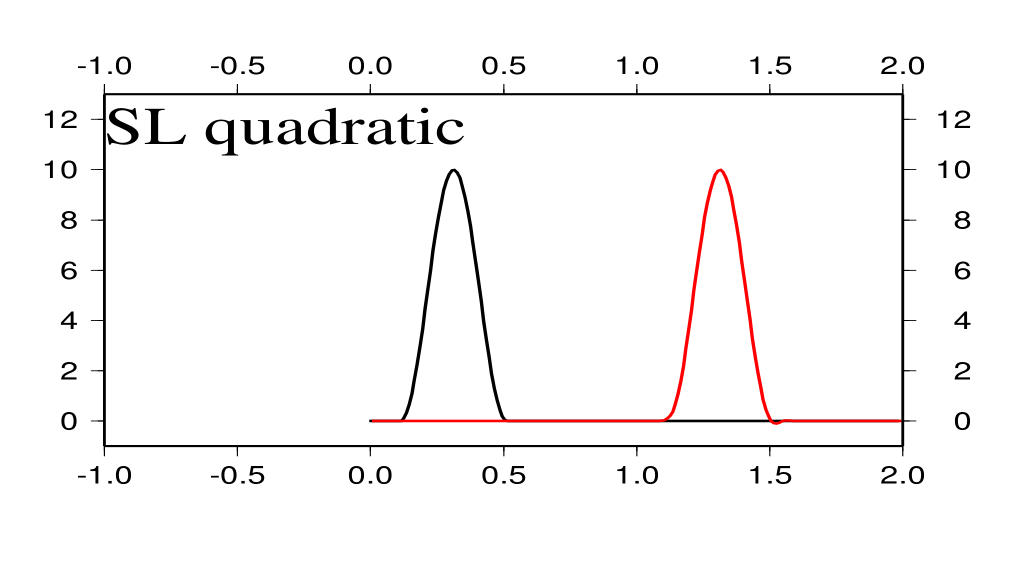
\includegraphics[width=0.8\textwidth,height=0.5\textwidth]{images/6_2}
	\caption{Полулагранжевый метод, точные траектории, квадратичная интерполяция}
	\label{img:6_2}
\end{figure}
%
%
\begin{figure}[ht] 
	\centering
	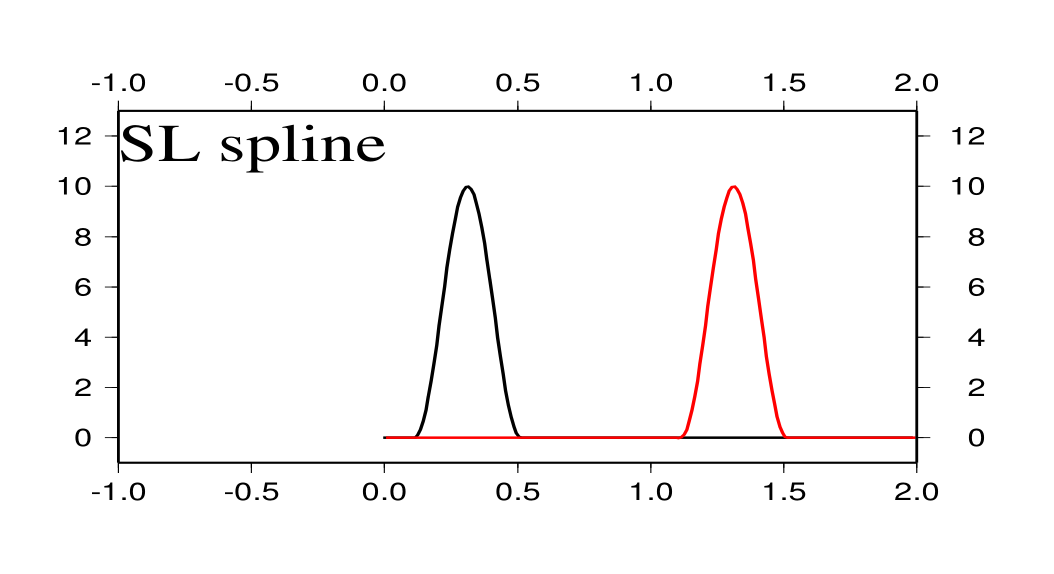
\includegraphics[width=0.8\textwidth,height=0.5\textwidth]{images/6_3}
	\caption{Полулагранжевый метод, точные траектории, кубическая интерполяция сплайнами}
	\label{img:6_3}
\end{figure}
%
\begin{table} [htbp]
	\centering
	\captionsetup{width=15cm}
	\caption{Ошибки полулагранжевого метода для одномерного теста.}\label{tbl:6_1}%
	\begin{tabular}{| p{2cm} || p{2cm} | p{2cm} | p{2.5cm} | p{2.5cm} | p{2.5cm}l |}
		\hline
		\hline
		Method   & \centering $e_2^{rel}$ & \centering $e_1^{rel}$ & \centering Dispersion & \centering Diffusion & \centering Minimum &\\
		\hline
		Linear     &\centering 6.31e-2 &\centering 7.40e-2 &\centering 3.84e-2  &\centering 2.13e-2 &\centering 0.0     &\\
		Quadratic  &\centering 7.98e-3 &\centering 9.38e-3 &\centering 9.55e-4  &\centering 4.36e-7 &\centering -0.1    &\\
		Spline     &\centering 5.02e-4 &\centering 3.60e-4 &\centering 3.77e-6  &\centering 3.57e-9 &\centering -9.5e-3 &\\
		\hline
		\hline
	\end{tabular}
\end{table}
%

Более квантифицируемый анализ представлен в таблице \ref{tbl:6_1}. В ней приведены относительные ошибки $l_1$ и $l_2$, которые на временном слое $n$ рассчитываются как
%
\begin{align}
\label{eq:equation6_1}
e_1^{rel}&=\frac{\sum_{i=1}^{N}|c_i^n-ex_i|}{\sum_{i=1}^{N}|ex_i|}\\
\label{eq:equation6_2}
e_2^{rel}&=\frac{\sqrt{\sum_{i=1}^{N}{(c_i^n-ex_i)}^2}}{\sqrt{\sum_{i=1}^{N}{ex_i}^2}}
\end{align}
%
где $c(x.t)$ это аналитическое решение, $ex_i=c(x_i,t^n)$ и $N$ это общее число точек вычислительной области. Также приведены дисперсионные и диффузионные ошибки. Данные величины были введены в~\cite{A69} и могут быть определены как
%
\begin{align}
	\label{eq:equation6_3}
   Dispersion\; error&=2\Big[\sigma(c^n)\sigma(ex)-\frac{1}{N^2}\sum_{i,j=1}^{N}(c_i^n-\bar{c})(ex_j-\bar{ex})\Big]\nonumber \\ 
    (\mathbf{????})Dissipation\;error&=[\sigma(c^n)-\sigma(ex)]^2+(\bar{c^n}-\bar{ex})^2,
\end{align}
%
где для общих сеточных функций $\phi_i$ определено
%
\begin{equation}
\label{eq:equation6_4}
\bar{\phi}=\frac{1}{N}\sum_{i=1}^{N}\phi_i\quad\sigma(\phi)^2=\frac{1}{N}\sum_{i=1}^{N}(\phi_i-\bar{\phi})^2.
\end{equation}
%
Они обладают свойством
%
\begin{equation}
\label{eq:equation6_5}
\sum_{i=1}^{N}(c_i^n-ex_i)^2=Dispersion\;error\,+\,Diffusion\;error,
\end{equation}
%
таким образом общая ошибка $l_2$ может быть разложена на два члена. Первая учитывает разницу между первыми двумя моментами вычисленного и точного решения. Этот член называется диффузионной ошибкой, потому что наибольший вклад в разности вносит численная диффузия рассматриваемого метода. Другой член измеряет разницу между корреляцией приближенного и точного решений и произведением их дисперсий. Если отклонение среднего между приближенным и точным решением это независимые случайные значения, данный член будет равен нулю. Таким образом, значения отличные от нуля означают пространственную корреляцию между данными отклонениями, а значит определенный фазовый сдвиг между вычисленным и точным решениями. Данные величины весьма полезны для аккуратной оценки свойств численного метода решения уравнения переноса. В довершение к этому, с целью обратить внимание на то, что имеют место вылеты и вбросы решения, минимум вычисленного решения также приведен в таблице.
\section*{Двумерная адвекция} \label{sect6_2}
Для случая двумерного пассивного переноса, мы рассмотрели наиболее простой и широко известный тестовый пример, а именно, вращение твердого тела. Вращение происходит вокруг центра вычислительной области $[0,2]\times[0,2]$,  в качестве начальных данных выбрана финитная колоколообразная функция $\mathcal{C}^1$ с максимальным значением равным 10. Период вращения был взят $T=1000$, шаг по пространству $\Delta x = 1/25$. Для первых экспериментов, шаг по времени был взят $\Delta t = 5.0$. Максимальные числа Куранта были получены $C=0.78$, таким образом условие КФЛ выполняется на всей вычислительной области. Тест выполнялся до времени $T=1000$. В первую очередь, на рис. \ref{img:6_4} показаны точные траектории, а также результаты, полученные при помощи полулагранжевого метода и кубической интерполяции сплайнами.
%
\begin{figure}[ht] 
	\centering
	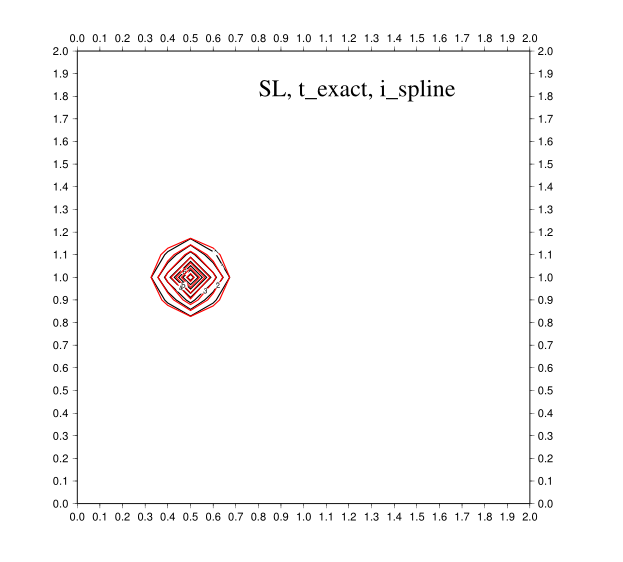
\includegraphics[width=0.8\textwidth,height=0.8\textwidth]{images/6_4}
	\caption{Полулагранжевый метод, точные траектории, кубическая интерполяция сплайнами}
	\label{img:6_4}
\end{figure}
%
%
\begin{figure}[ht] 
	\centering
	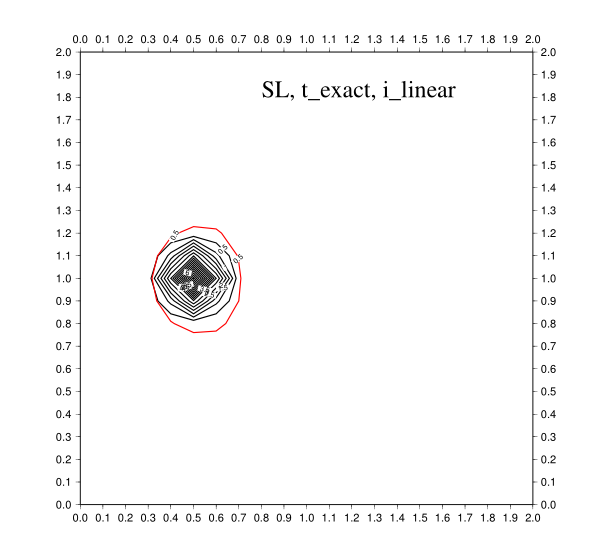
\includegraphics[width=0.8\textwidth,height=0.8\textwidth]{images/6_5}
	\caption{Полулагранжевый метод, точные траектории, билинейная интерполяция}
	\label{img:6_5}
\end{figure}
%
%
\begin{table} [htbp]
	\centering
	\captionsetup{width=15cm}
	\caption{Ошибки полулагранжевого метода с точным интегрированием траекторий в эксперименте вращения твердого тела.}\label{tbl:6_2}%
	\begin{tabular}{| p{4cm} || p{2cm} | p{2cm} | p{2cm} | p{2.5cm} | p{2.5cm}l |}
		\hline
		\hline
		\centering Method   &\centering $e_2^{rel}$ &\centering $e_1^{rel}$ &\centering Dispersion &\centering Diffusion &\centering Minimum & \\
		\hline
		\centering Bilinear &\centering 0.89 &\centering 1.51 &\centering 0.49  &\centering 0.75 &\centering 0.0     & \\
		\centering Cubic    &\centering 0.21 &\centering 0.35 &\centering 4.31e-2  &\centering 2.76e-3 &\centering -0.98    & \\
		\hline
		\hline
	\end{tabular}
\end{table}
%
%
\begin{figure}[ht] 
	\centering
	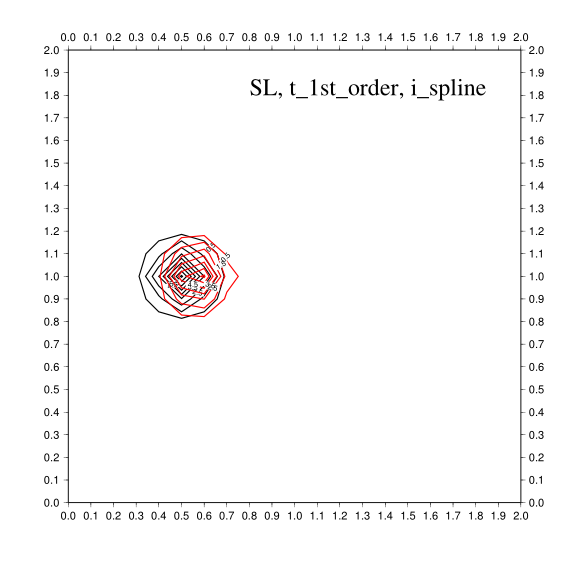
\includegraphics[width=0.8\textwidth,height=0.8\textwidth]{images/6_6}
	\caption{Полулагранжевый метод, метод Эйлера для траекторий, интерполяция сплайнами}
	\label{img:6_6}
\end{figure}
%
%
\begin{table} [htbp]
	\centering
	\captionsetup{width=15cm}
	\caption{Ошибки полулагранжевого метода с приближенным интегрированием траекторий в эксперименте вращения твердого тела.}\label{tbl:6_3}%
	\begin{tabular}{| p{4cm} || p{2cm} | p{2cm} | p{2cm} | p{2.5cm} | p{2.5cm}l |}
		\hline
		\hline
		\centering Method   &\centering $e_2^{rel}$ &\centering $e_1^{rel}$ &\centering Dispersion &\centering Diffusion &\centering Minimum & \\
		\hline
		\centering Cubic, 1st               &\centering 0.62 &\centering 0.75 &\centering 0.54     &\centering 4.58e-2 &\centering  -0.27   & \\
		\centering Cubic, 1st, $\Delta t/5$   &\centering 0.19 &\centering 0.31 &\centering 5.06e-2  &\centering 3.62e-3 &\centering -0.43   & \\
		\centering Cubic, 2nd               &\centering 0.14 &\centering 0.23 &\centering 2.93e-2  &\centering 2.84e-3 &\centering -0.23   & \\
		\hline
		\hline
	\end{tabular}
\end{table}
%
%
\begin{figure}[ht] 
	\centering
	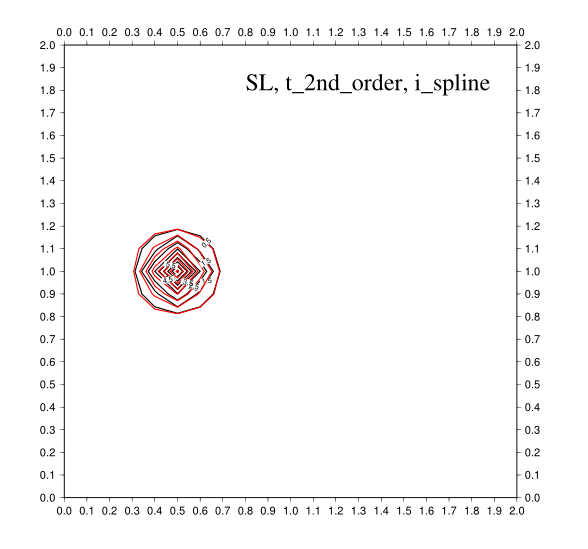
\includegraphics[width=0.8\textwidth,height=0.8\textwidth]{images/6_7}
	\caption{Полулагранжевый метод, метод Рунге"--~Кутта второго порядка, интерполяция сплайнами}
	\label{img:6_7}
\end{figure}
%
%
\begin{figure}[ht] 
	\centering
	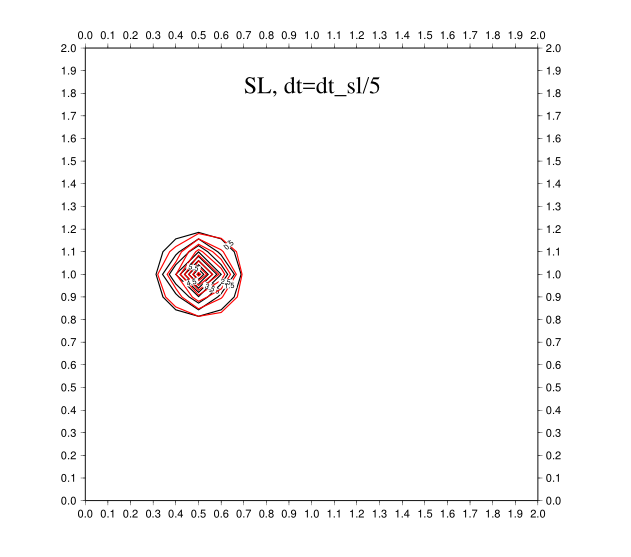
\includegraphics[width=0.8\textwidth,height=0.8\textwidth]{images/6_8}
	\caption{Полулагранжевый метод, метод Эйлера для траекторий с $\Delta t/5$, интерполяция сплайнами}
	\label{img:6_8}
\end{figure}
%
%
\begin{table} [htbp]
	\centering
	\captionsetup{width=15cm}
	\caption{Ошибки методов Эйлера в одномерном эксперименте.}\label{tbl:6_4}%
	\begin{tabular}{| p{5cm} || p{2cm} | p{2cm} | p{2cm} | p{2cm} | p{2cm}l |}
		\hline
		\hline
		\centering Method   &\centering $e_2^{rel}$ &\centering $e_1^{rel}$ &\centering Dispersion &\centering Diffusion &\centering Minimum & \\
		\hline
		\centering upwind                     &\centering 0.23    &\centering 0.29    &\centering 0.54     &\centering 0.3      &\centering  0.0      & \\
		\centering leapfrog                   &\centering 3.62e-2 &\centering 4.94e-2 &\centering 1.96e-2  &\centering 8.25e-11 &\centering -0.33     & \\
		\centering Lax Wendroff               &\centering 3.47e-2 &\centering 4.44e-2 &\centering 1.8e-2   &\centering 1.18e-5  &\centering -0.3      & \\
		\centering Crowley                    &\centering 2.48e-3 &\centering 2.23e-3 &\centering 9.25e-5  &\centering 1.7e-9   &\centering -4.2e-2   & \\
		\centering leapfrog, 4th order in $x$   &\centering 1.18e-2 &\centering 1.54e-2 &\centering 2.11e-3  &\centering 3.57e-10 &\centering -0.13     & \\
		\hline
		\hline
	\end{tabular}
\end{table}
%
%
\begin{table} [htbp]
	\centering
	\captionsetup{width=15cm}
	\caption{Ошибки методов Эйлера в эксперименте с вращением твердого тела.}\label{tbl:6_5}%
	\begin{tabular}{| p{4cm} || p{2cm} | p{2cm} | p{2.5cm} | p{2.5cm} | p{2cm}l |}
		\hline
		\hline
		\centering Method   &\centering $e_2^{rel}$ &\centering $e_1^{rel}$ &\centering Dispersion &\centering Diffusion &\centering Minimum & \\
		\hline
		\centering Crowley $\Delta t / 5$              &\centering 0.55 &\centering 1.4  &\centering 0.46    &\centering 2.75e-3  &\centering -2.73   & \\
		\centering Crowley $\Delta t / 5\;\Delta x/2$  &\centering 0.16 &\centering 0.27 &\centering 4.03e-2 &\centering 3.95e-4  &\centering -0.65   & \\
		\hline
		\hline
	\end{tabular}
\end{table}
%
\section*{Сравнение с простыми схемами Эйлера} \label{sect6_3}
Вопрос являются ли полулагранжевые схемы более предпочтительными, чем схемы Эйлера, в качестве подхода к адвективным задачам, обсуждается весьма широко. В данном обзоре представлен всего лишь небольшой вклад в этот долгий и ожесточенный спор. Целью данного вклада является попытка предоставить несколько примеров типовых результатов, получаемых после применения указанных схем к стандартному набору экспериментов.

Прежде всего, представлены результаты простейших одномерных адвективных схем для теста с пассивной формой адвекции, который обсуждался в разделе 6.1. Число Куранта было выбрано $C=1/2$  с тем, чтобы удовлетворить условию Куранта"--~Фридрихса"--~Леви. Были использованы адвективные схемы, обсуждавшиеся в разделе 2. В эксперименте с вращением твердого тела для разных шагов по времени и пространству была применена двумерная схема Кроули четвертого порядка, полученная путем простой дискретизации производных по направлениям $x$ и $y$. С целью получения приемлемых результатов применялись более мелкие шаги по времени, нежели в тестах для полулагранжевого подхода. Отношение шага по времени к шагу, применявшегося в тестах для полулагранжевого подхода, отображено на легенде иллюстраций.
%

Сделать окончательные выводы на основе настолько скромных и не исчерпывающих экспериментов не представляется возможным. Однако, по мнению автора данного обзора, все же возможно предоставить некоторые соображения по этому поводу. Во-первых, налицо уменьшение дисперсионной ошибки в случае применения точных методов, основанных на схеме набегающего потока. Подобные результаты можно увидеть для одномерных экспериментов как при использовании эйлеровых схем набегающего потока, таких как метод Кроули, так и для полулагранжевого метода. Схема Кроули (на основе схемы набегающего потока), также как и схема с перешагиванием четвертого порядка \eqref{eq:equation2_5}, формально имеют одинаковый порядок точности по пространству, однако, при этом, методы, основанные на схеме набегающего потока, показывают лучшие результаты.

Очевидно также, что сравнения результатов одномерных экспериментов в действительности недостаточно, поскольку, как представляется, другой ключевой особенностью полулагранжевых методов является многомерность. В одномерном случае, схема Кроули формально имеет тот же порядок точности, что и полулагранжевый метод с траекториями, аппроксимированными методом первого порядка и кубической интерполяцией сплайнами. Однако, прямое обобщение на два измерения очевидно является менее точным. Существуют полностью многомерные, точные эйлеровы схемы (см., например, среди многих других~\cite{A32},~\cite{A64},~\cite{A66}), но требуемые вычислительные затраты и сложность, как представляется, имеют тот же порядок роста (как минимум), как и те, которых требуют обычные полулагражевые методы.

Представленные соображения никак не затрагивают безусловную устойчивость полулагранжевых схем и сопутствующую тему для дискуссий. Очевидно, что возможность работать с моделями, которые содержат большие числа Куранта, очень заманчива, особенно для моделей предсказания погоды, использующих широтно-долготные декартовы сетки (latitude-longitude cartesian meshes), где сходимость меридианов на полюсах естественным образом приводит к значительным КФЛ-ограничениям для эйлеровых схем. С другой стороны, злоупотребление безусловной устойчивостью может также привести к другим проблемам с точностью, как, например, обсуждается в\cite{A2},~\cite{A26}.

Сводя всё воедино, кажется, что замена противоречия \textit{эйлеровы vs. полулагранжевы} на противоречие \textit{наивные vs. полностью многомерные} может иметь некоторый смысл. С точки зрения концепции, носящей довольно общий характер, предложенной, например, в~\cite{A43}, озвученная замена представляется оправданной по отношению к соответственному противоречию для проблемы сохранения массы. Проблема эффективности потребует намного более аккуратных и комплексных сравнений (чьи результаты, вероятно, могут дать противоречивые ответы, зависящие от целевого приложения). Однако, следует отметить, что, как указано в~\cite{A26}, числа Куранта часто меньше единицы в большей части вычислительной области. Таким образом, это особенный выигрыш в надежности, который обеспечивают полулагранжевые методы, позволяя работать с числами Куранта больше единицы. (Thus, it is especially a gain of robustness that is provided by semi-Lagrangian methods, by enabling \textit{cum grano salis} runs with Courant numbers larger than one somewhere).
%
\begin{figure}[ht] 
	\centering
	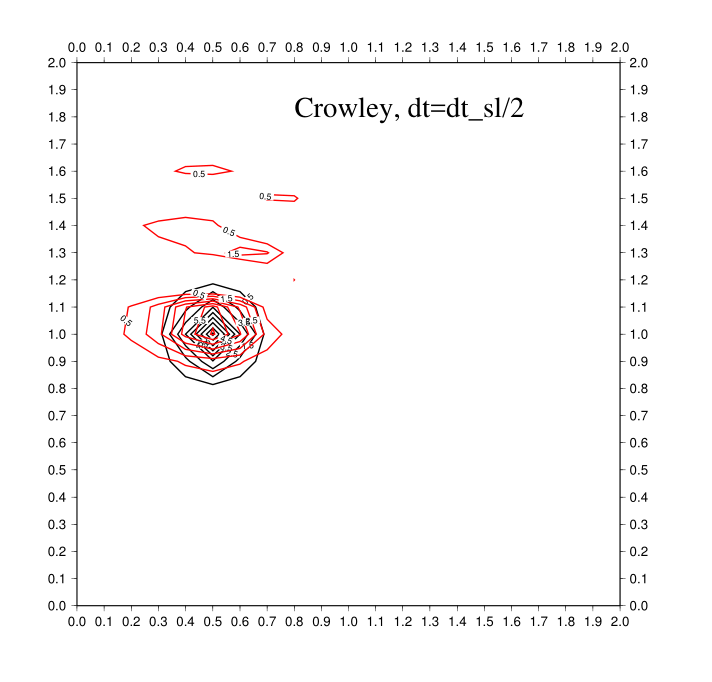
\includegraphics[width=0.8\textwidth,height=0.8\textwidth]{images/6_9}
	\caption{Метод Эйлера (Кроули) для $\Delta t/2$}
	\label{img:6_9}
\end{figure}
%
%
\begin{figure}[ht] 
	\centering
	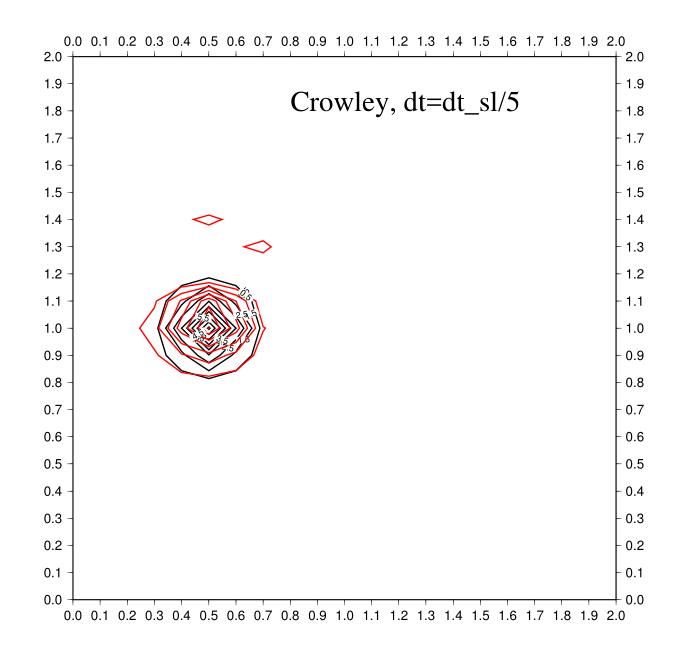
\includegraphics[width=0.8\textwidth,height=0.8\textwidth]{images/6_10}
	\caption{Метод Эйлера (Кроули) для $\Delta t/5$}
	\label{img:6_10}
\end{figure}
%
%
\begin{figure}[ht] 
	\centering
	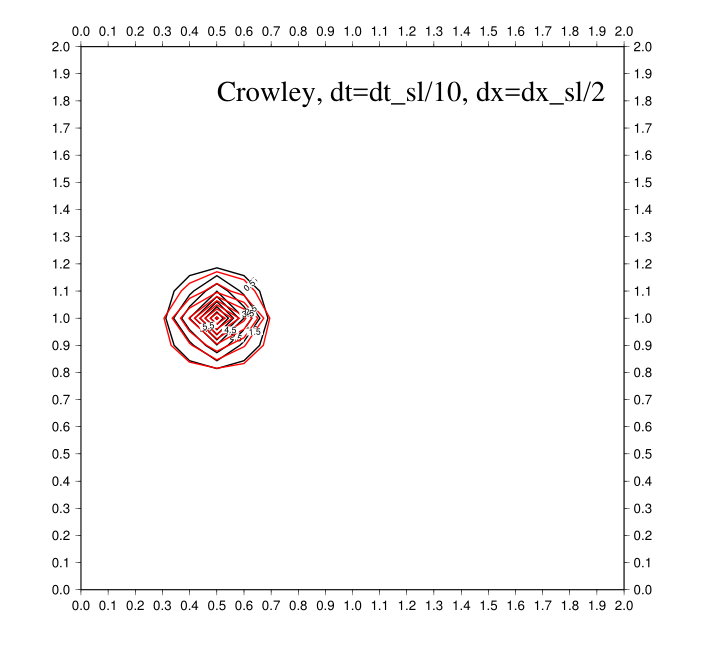
\includegraphics[width=0.8\textwidth,height=0.8\textwidth]{images/6_11}
	\caption{Метод Эйлера (Кроули) для $\Delta t/10$ и $\Delta x/2$}
	\label{img:6_11}
\end{figure}
%
\chapter{Теория полулагранжевых методов: анализ сходимости и устойчивости} \label{chapt_7}
Весьма занимательно, что одной из особенностей, которая, на сегодняшний день, наиболее тесно ассоциируются с полулагранжевыми методами, то есть сохранение устойчивости для любого значения числа Куранта, не была ясно распознана на ранних стадиях разработки данных методов (см., например,~\cite{A30},~\cite{A53}). Результаты работ А. Роберта~\cite{A59},\cite{A60} сподвигли доказать безусловную сходимость по Нейману для линейной и квадратичной интерполяции в~\cite{A3}, а также в~\cite{A52} для кубической интерполяции сплайнами, таким образом расширив предыдущие результаты из~\cite{A53}. Сходимость в общем случае и анализ устойчивости для случая адвекции с переменными коэффициентами был представлен в~\cite{A16}. Подходы, использующие характеристический метод Галёркина, были проанализированы в~\cite{A44},~\cite{A68}, а основная концепция анализа методов на основе характеристик для неструктурированных сеток была предложена в~\cite{A43}.

Анализ устойчивости в~\cite{A16} расширяет предыдущие результаты на более общие техники интерполирования, в частности на те, которые присущи конечно-элементным методам. Там же, проведен анализ сходимости для конечно-элементной формулировки полулагранжевого метода, использующего методы Рунге"--~Кутта для аппроксимации траекторий в случае для которых достаточно единичного шага (т.е. число Куранта меньше единицы). Один из основных результатов в~\cite{A16} может быть обобщен и переформулирован в виде теоремы в контексте конечно-разностной формулировки, кратко изложенной в разделе 2.
%
\begin{theorem}
	Обозначив метод аппроксимации траектории как $\mathcal{O}(\Delta t^p)$, ошибку  метода интерполяции по пространству как $\mathcal{E}(\Delta x)$ и определив временной интервал $[0,T]$ таким образом, что $\Delta t=T/N$, при условии достаточной регулярности (under mild regularity conditions) выполняется следующее
\begin{equation}
\max_{n=1,N} \max_{i}|c(x_i,t^n)-c_i^n| \le C\Big[\mathcal{O}(\Delta t^p)+ N\mathcal{E}(\Delta x)\Big].
\end{equation}
\end{theorem}
%
%
\begin{table} [htbp]
	\centering
	\captionsetup{width=15cm}
	\caption{Тест сходимости полулагранжевого метода и метода Лакса"--~Вендроффа (одномерное уравнение переноса).}\label{tbl:7_1}%
	\begin{tabular}{| p{3.5cm} || p{4cm} | p{4cm} | p{3.5cm}l |}
		\hline
		\hline
		&\centering Ошибка $l_2$ &\centering ошибка $l_2\; \Delta t/2, \Delta x/2$ &\centering Порядок & \\
		\hline
		\centering SL, cubic    &\centering 1.96e-2    &\centering 4.72e-3   &\centering 2.2 & \\		
		\centering Lax Wendroff &\centering 0.13       &\centering 3.58e-2   &\centering 1.8 & \\
		\hline
		\hline
	\end{tabular}
\end{table}
%
%
\begin{table} [htbp]
	\centering
	\captionsetup{width=15cm}
	\caption{Тест сходимости полулагранжевого метода (одномерное уравнение переноса).}\label{tbl:7_2}%
	\begin{tabular}{| p{3.5cm} || p{4cm} | p{4cm} | p{3.5cm}l |}
		\hline
		\hline
		&\centering Ошибка $l_2$ &\centering ошибка  $l_2\;\Delta t/2$ &\centering Порядок & \\
		\hline
		\centering SL, cubic              &\centering 1.96e-2    &\centering 2.27e-2  &\centering -0.5 & \\		
		\centering SL, cubic $\Delta x/2$ &\centering 3.19e-4       &\centering 4.72e-3   &\centering -3.9 & \\
		\hline
		Порядок &\centering 5.9     &\centering 2.2   &\centering  & \\
		\hline
		\hline
	\end{tabular}
\end{table}
%
Здесь $x_i$ это узлы декартовой сетки дискретизации в $\mathbf{R}^d$. Можно увидеть, что максимальное значение нормы $l_{\infty}$ растет пропорционально числу шагов по времени. Хотя это не строгая оценка сверху, можно легко увидеть накопление ошибки в простых адвективных тестах. Для более ясной демонстрации влияния интерполяционной ошибки $\mathcal{E}(\Delta x)$, см., например, результаты на рис.~\ref{img:6_4},~\ref{img:6_5}. Последствия данного свойства заключаются в том, что тесты на сходимость дают скорее нелепые, а то и разочаровывающие результаты, см., например, таблицу~\ref{tbl:6_2}, результаты представленные в~\cite{A16} и обсуждение~\cite{A26}. Как пример, в таблице~\ref{tbl:7_1} приведены результаты экспериментов для простой адвекции для полулагранжевой схемы и схемы Лакса"--~Вендроффа. Здесь рассмотрена одномерная адвекция, a шаги по времени и пространству были одновременно уменьшены вдвое. В то время как схема Лакса"--~Вендроффа показывает скорость сходимости, которая примерно соответствующей ожидаемой, скорость сходимости (формально метода четвертого порядка по пространству) полулагранжевой схемы едва ли около двух. Эти результаты могут быть противопоставлены результатам из таблицы~\ref{tbl:7_2}, где тот же самый тест был проведен с поочередным уменьшением вдвое шага по пространству и времени. Можно увидеть, что увеличение пространственного разрешения приводит к последовательному уменьшению ошибки дискретизации, даже за пределами ожидаемой скорости сходимости, в то время как уменьшение вдвое шага по времени приводит, как оказалось, к росту ошибки (следовательно, к отрицательным скоростям сходимости), скорость которого, однако, зависит от пространственного разрешения.
\chapter{Полулагранжевые методы против метода характеристик: полунеявные полулагранжевые методы для условий с малым числом Фруда} \label{chapt_8}
Полулагранжевый метод и метод характеристик во многих аспектах очень похожи.
Например, метод  Куранта, Айзексона и Риз~\cite{A11}, использованный к скалярному уравнению переноса дает вариант полулагранжевого метода. С другой стороны, если рассматривать приложение к гиперболическим системам, то способ которым в общем случае применяют полулагранжевый метод к решению атмосферных уравнений движения в метеорологической литературе весомо отличается от метода характеристик. В этом разделе, будет кратко рассмотрен метод характеристик и будут обозначены отличия от полуявного, полулагранжевого метода.

Литература по характеристическим методам не будет рассмотрена здесь в полной мере, приведены некоторые релевантные ссылки на литературу, где данные методы рассматриваются в близком отношении к полулагранжевым методам, например,~\cite{A17},~\cite{A18},~\cite{A19},~\cite{A41},~\cite{A42},~\cite{A44}.

Рассмотрим одномерную линейную гиперболическую систему
%
\begin{equation}
\label{eq:equation8_1}
\frac{\partial\mathbf{c}}{\partial t} + \mathbf{A}\frac{\partial \mathbf{c}}{\partial{x}} = 0,
\end{equation}
%
где гиперболичность означает, что $\mathbf{A}$ имеет действительные неодинаковые собственные значения, а также невырожденную матрицу $T$, чьи столбцы содержат собственные числа матрицы $\mathbf{A}$ и верно, что 
$\mathbf{T}^1\mathbf{A}\mathbf{T}=\mathbf{\Lambda}$, где $\mathbf{\Lambda}$ это диагональная матрица собственных чисел $\mathbf{A}$. Для определенности и для последующего обсуждения, рассмотрим линейные уравнения мелкой воды, для которых
%
\begin{equation*}
\mathbf{c} = \begin{bmatrix}
h \\
u
\end{bmatrix}
 \quad
\mathbf{A} = \begin{bmatrix}
	U & H\\
	g & U
\end{bmatrix}
\end{equation*}
%
таким образом
%
\begin{equation*}
\mathbf{\Lambda} = \begin{bmatrix}
U + \sqrt{gH} & 0\\
0 & U - \sqrt{gH}
\end{bmatrix}
\quad
\mathbf{T} = \begin{bmatrix}
\frac{1}{2} & \frac{1}{2}\sqrt{\frac{H}{g}}\\
\frac{1}{2}  & -\frac{1}{2} \sqrt{\frac{H}{g}}
\end{bmatrix}
\quad
\mathbf{T}^{-1} = \begin{bmatrix}
1 & 1\\
\sqrt{\frac{g}{H}}  & -\sqrt{\frac{g}{H}}
\end{bmatrix}
\end{equation*}
%
Полагая $\mathbf{d}=\mathbf{T}\mathbf{c}$ и производя замену переменных в~\eqref{eq:equation8_1} получим
%
\begin{equation}
\label{eq:equation8_2}
\frac{\partial\mathbf{d}}{\partial t} + \mathbf{\Lambda}\frac{\partial \mathbf{d}}{\partial{x}} = 0.
\end{equation}
%
Теперь полученная система состоит из двух независимых (decoupled), одномерных уравнений адвекции.
Метод Куранта, Айзексона и Риса~\cite{A11} решает их на каждом временном шаге, опуская траекторию назад во времени и интерполируя на шаг характеристики. Значения исходных переменных затем могут быть восстановлены как $\mathbf{c}=\mathbf{T}^{-1}\mathbf{d}$. В линейном случае, метод вернет
%
\begin{align}
\label{eq:equation8_3}
h_i^{n+1}&=\frac{1}{2}h_{i-\frac{(U+\sqrt{gH})\Delta t}{\Delta x}}^n+h_{i-\frac{(U-\sqrt{gH})\Delta t}{\Delta x}}^n \nonumber \\ 
u_i^{n+1}&=\frac{1}{2}u_{i-\frac{(U+\sqrt{gH})\Delta t}{\Delta x}}^n+u_{i-\frac{(U-\sqrt{gH})\Delta t}{\Delta x}}^n
\end{align}
%
Здесь используется та же нотация, которая использовалась в разделе 2.

Поскольку уравнения Эйлера и уравнения мелкой воды также составляют гиперболическую систему, в принципе, возможно применять метод характеристик напрямую к атмосферному моделированию. Однако, ряд особенностей уравнениях атмосферного движения~\eqref{eq:equation3_1}-~\eqref{eq:equation3_3} вместо этого приводит к совершенно иным результатам в атмосферном моделировании. Масштабный анализ, описанный в разделе 3, показывает, что крупномасштабные атмосферные потоки находятся в приближенном геострофическом равновесии далеко от тропиков (away from tropics). Это также выполняется для упрощенных двумерных моделей, таких как уравнения мелкой воды, для которых геострофический баланс можно выразить как 
%
\begin{equation}
\label{eq:equation8_4}
-g\nabla h - f\mathbf{k}\times\mathbf{v}\approx 0.
\end{equation}
%
Таким образом, сила Кориолиса является очень важной частью уравнений, однако она приблизительно равна нулю (имеет почти нулевой порядок), уравнение~\eqref{eq:equation8_4} не отображено в соответствующей гиперболической системе и не влияет на характеристики. Более того, поворотный компонент (the rotational component) типичного крупномасштабного потока примерно на один порядок величины больше, чем компонента дивергенции (см., например, [24], [49]). Как результат, могут быть разработаны новые упрощенные модели, такие как квазгеострофические модели или модели на основе баротропического уравнения завихренности, которые все еще учитывают базовые наблюдаемые явления крупномасштабных потоков. Таких моделях больше нет гравитационных волн (т.е. гравитационные волны это решения уравнений мелкой воды, чьи особенности связаны с характеристиками соответствующей гиперболической системы). Некоторые наиболее подходящие физические величины, определяющие атмосферные потоки (например, потенциальная завихренность) просто адвектируются полем скоростей, нежели чем распространяются вдоль характеристик. В случае полных уравнений Эйлера ~\eqref{eq:equation3_1}-~\eqref{eq:equation3_3}, решения определяются характеристиками связанной гиперболической проблемы (т.е. звуковыми волнами), которые, вообще говоря, невозможно получить даже на сетках с очень мелким шагом по пространству. Более того, предыдущий анализ показывает, что они не являются самым точным термом для предсказания крупномасштабных потоков. Даже для предсказания мезомасштабных особенностей, они намного менее точны (релевантны), чем интервальные гравитационные волны, порожденные эффектами подъемной силы, которые также в основном зависят от термов, которые не несут вклад в характеристики уравнений Эйлера. Также следует учесть, что типичные атмосферные приложения имеют дело с потоками с небольшим значением числа Маха и в квазинесжимаемом режиме, то есть, в условиях линейных уравнений мелкой воды, режимы для которых
%
\begin{equation}
\label{eq:equation8_5}
\frac{|U|}{\sqrt{gH}} \ll 1.
\end{equation}
%
Таким образом, характеристики полученные из гиперболической системы слега отличаются от линий тока потока, вдоль которых соответствующие величины адвектируются фактически. В добавок ко всем этим проблемам, наиболее стандартные реализации метода характеристик обязаны удовлетворять условию Куранта"--~Фридрихса"--~Леви следующего вида
%
\begin{equation}
\label{eq:equation8_6}
\frac{|U\pm\sqrt{gH}|\Delta t}{\Delta x}.
\end{equation}
%
Таким образом, если выполнено~\eqref{eq:equation8_5} данные дискретизации по времени весьма неэффективны для предсказания гравитационных волн.

Полунеявные, полулагранжевые методы, которые были предложены Робертом в~\cite{A60} не страдают от наличия ограничения на устойчивость, что объясняет их широкое (хотя, ни в коем случае не универсальное) использование, особенно для моделей предсказания погоды. В полунеявном, полулагранжевом подходе, лагранжевы производные, например в уравнениях~\eqref{eq:equation3_4}-~\eqref{eq:equation3_5}, аппроксимируются конечной разностью вдоль аппроксимированной линии тока, в то время, как члены, ответственные за распространение гравитационных волн дискретизируются неявно по времени с целью избежать ограничения на устойчивость~\eqref{eq:requation8_6}. Более точно, используя нотацию, введеную в разделе 2, рассмотрим для каждой общей точки $\mathbf{x}$ в вычислительной области, следуюшее ОДУ
% 
\begin{equation}
\label{eq:equation8_7}
\frac{d}{ds}\mathbf{X}(s;s+\Delta t,\,\mathbf{x})=\mathbf{u}(\mathbf{X}(s;s+\Delta t,\,\mathbf{x}), s)
\end{equation}
%
и возьмем $\mathbf{x}_{*}=\mathbf{X}(t; t + \Delta t,\,x).$ 2 $\phi_*$. Более того, обозначим $\phi_*$ общую величину, которая интерполирована на точке $\mathbf{x}_*$. Полунеявная полулагранжева дискретизация уравнений мелкой воды представлена как
%
\begin{align}
\label{eq:equation8_8}
\frac{h^{n+1}-h_{*}^n}{\Delta t}&=-\frac{1}{2} [h^n\nabla \cdot \mathbf{v}^{n+1} + h_*^n \nabla \cdot \mathbf{v}_{*}^n] \\
\label{eq:equation8_9}
\frac{\mathbf{v}^{n+1}-\mathbf{v}_{*}^n}{\Delta t}&=-\frac{g}{2}[\nabla h^{n+1}+\nabla h_{*}^n] - \frac{f\mathbf{k}\times\mathbf{v}^{n+1}+f_{*}\mathbf{k}\times\mathbf{v}_{*}^n}{2}.
\end{align}
%
Как было отмечено ранее, лагранжевы производные аппроксимируются обратными конечными разностями вдоль линий тока (backward finite differences along the streamlines), в то время, как члены ответственные за распространение гравитации и инертно-гравитационных волн (inertia-gravity waves) (см., например,~\cite{A49}) усредняются по времени вдоль линий тока. Алгоритм невявной дискретизации, получившийся из~\eqref{eq:equation8_8}-~\eqref{eq:equation8_9} влечет за собой подстановку уравнения~\eqref{eq:equation8_9} в~\eqref{eq:equation8_8} с целью получить эллиптическое уравнение для $h^{n+1}$, которое должно решаться на каждом временном шаге. Когда это значение вычислено, осуществляется обратная подстановка в~\eqref{eq:equation8_9}, чтобы завершить алгоритм дискретизации по времени. Анализ фон Неймана для соответствующих линеаризированных уравнений показывает, что данная дискретизация по времени безусловно устойчива. Более того, она может быть успешно расширена на полные уравнения Эйлера.
\chapter{Консервативные (mass conservative) и векторные (flux form) полулагранжевые методы} \label{chapt_9}
Вообще говоря, полулагражевые методы в той формулировке, которая была представлена в данном обзоре, не сохраняют массу. В качестве примера, рассмотрим одномерный и двумерный эксперименты, обсуждавшиеся ранее. Отношения массы рассчитанного решения и начального представлены в таблицах~\ref{tbl:9_1} и~\ref{tbl:9_2} для одномерного и двумерного случаев, соответственно.

Было предложено несколько подходов с целью преодолеть недостаточную консервативность полулагранжевых методов в отношении сохранения масс. Во многих практических приложениях используется постериорное восстановление масс с целью сохранить массу в атмосфере постоянной. Методы, предложенные в~\cite{A23},~\cite{A51}, являют своей целью именно выполнение закона сохранения масс, которое, однако, по-прежнему достигается путем перераспределения потерь и приростов массы среди всех точек сетки. Ни один из простых подходов не гарантирует выполнения локального закона сохранения, т. е. изменения решения в данной точке сетки не обязательно зависит от значений в соседних узлах сетки.
%
\begin{table} [htbp]
	\centering
	\captionsetup{width=15cm}
	\caption{Ошибка полулагранжевого методы по отношению к закону сохранения масс одномерного теста (число Куранта 2.5).}\label{tbl:9_1}%
	\begin{tabular}{| p{3.5cm} || p{4cm} | p{4cm} | p{3.5cm}l |}
		\hline
		\hline
		&\centering Linear &\centering Quadratic &\centering Spline & \\
		\hline
		Computed/exact mass &\centering 1.00002384  &\centering 1.00293481 &\centering 1.00027871 & \\		
		\hline
		\hline
	\end{tabular}
\end{table}
%
%
\begin{table} [htbp]
	\centering
	\captionsetup{width=15cm}
	\caption{Ошибка полулагранжевого методы по отношению к закону сохранения масс двумерного теста (число Куранта 0.7).}\label{tbl:9_2}%
	\begin{tabular}{| p{3.5cm} || p{4cm} | p{4cm} | p{3.5cm}l |}
		\hline
		\hline
		&\centering Linear, exact traj. &\centering Spline, 1st order traj. &\centering Spline, 2nd order traj. & \\
		\hline
		Computed/exact mass &\centering 0.7668  &\centering 0.8828 &\centering 1.1059 & \\		
		\hline
		\hline
	\end{tabular}
\end{table}
%

Для того, чтобы достичь выполнения локального закона сохранения применяют две основные стратегии. С одной стороны, уравнение переноса
%
\begin{equation}
\label{eq:equation9_1}
\frac{\partial c}{\partial t} + \mathbf{u}\cdot\nabla c = 0
\end{equation}
%
может быть проинтегрировано по объему $\Omega(t)$, который движется вместе с потоком, таким образом получая
%
\begin{equation}
\label{eq:equation9_2}
\frac{d}{dt} \int_{\Omega (t)} cdx = 0
\end{equation}
%
Полагая $\Omega (t + \Delta t)$ равным контрольному объему сетки (mesh control volume), как предполагается в не консервативном полулагранжевом методе, простая дискретизация по времени даёт
%
\begin{equation}
\label{eq:equation9_3}
\frac{d}{dt} \int_{\Omega (t+\Delta t)} cdx = \int_{\Omega (t)} cdx
\end{equation}
%
где $\Omega (t)$  это теперь передний по ходу объем сетки (upstream control volume), который трансформируется в $\Omega (t + \Delta t)$ за шаг $\Delta t$. Уравнение~\eqref{eq:equation9_3} затем приближенно вычисляется (is then discretized) путем приближенного восстановления переднего по ходу контрольному объему и приближенным вычислением интеграла в правой части. Этот подход иногда называют консервативным перераспределением или клеточно-интегрируемым полулагранжевым методом. Идея перераспределения восходит, по крайней мере, к~\cite{A25}. Варианты полулагранжевых методов, сохраняющих массу, основанные на этой концепции перераспределения были введены, например, в~\cite{A29},~\cite{A34},~\cite{A35},~\cite{A13},~\cite{A47}.

Альтернативный способ достичь выполнения локального закона сохранения наиболее близок по духу к конечно-объемным эйлеровым методам. Уравнение~\eqref{eq:equation9_1}, переписанное в виде закона сохранения
%
\begin{equation}
\label{eq:equation9_4}
\frac{\partial c}{\partial t} + \nabla\cdot(\mathbf{u}c) = 0
\end{equation}
%
при использовании уравнения неразрывности (для простоты, здесь рассмотрен несжимаемый поток с постоянной плотностью). Затем, как обычно принято, уравнение~\eqref{eq:equation9_4} интегрируют по пространству над фиксированным контрольным сеточным объемом $\Omega$, а затем применяют теорему Гаусса"--~Остроградского. Полученное уравнение интегрируется по времени с обычным шагом по времени, так, чтобы получить
%
\begin{equation}
\label{eq:equation9_5}
\int_{\Omega}c(x,\,t +\Delta t)dx=\int_{\Omega}c(x,\,t)dx-\int_{t}^{t+\Delta t}ds\int_{\partial\Omega}c(x,\,s)\mathbf{u}(x,\,s)\cdot\mathbf{n}
\end{equation}
%
Уравнение~\eqref{eq:equation9_5} дискретизируется путем приближенного восстановления потока через границы области на временном шаге $\Delta t$. Рассчитываются обратные полулагранжевые траектории, которые достигают ряда точек (некоторых точек) вдоль $\partial \Omega$ на шаге $t+\Delta t$, а затем используются для аппроксимации части потока, которая переносится через границы вычислительной области. Затем над этими точками осуществляется некоторая форма полиномиального восстановления, чтобы приблизить интеграл по области в правой части. Мы будем называть подобные методы потоковой формой полулагранжевых методов. Примеры подобных методов можно найти в~\cite{A17},~\cite{A18},~\cite{A19},~\cite{A31},~\cite{A33}. В~\cite{A43} данные подходы, наряду с анализом их устойчивости, описаны в более широком контексте, а именно как обобщенные методы Годунова. Следует отметить, что данный подход может быть также интерпретирован как естественное обобщение так называемых волновых методов (wave propogation methods), см., например,~\cite{A32}.
\newpage
\chapter{Выводы} \label{chapt_10}
Был представлен полулагранжевый метод решения уравнения переноса, а также рассмотрено его развитие в контексте атмосферного моделирования за последние 50 лет. Были рассмотрены его простейшие свойства и приведен обзор базовых теоретических свойств. В частности, предпринята попытка применить методы, разработанные для атмосферного моделирования, в более широкой перспективе современных методов конечных объемов и разностей, вместе с набросками предложенными К. В. Мортоном в~\cite{A43}. Возможно, осмысление сильно выраженных сходств между современными, полностью многомерными адвективными схемами поможет утихомирить многочисленные дебаты относительно достоинств эйлеровых и лагранжевых схем.
%\newpage